\section{Architectural Overview}
The Mobility Features Package will be used in a mobile-health application, which will then have access to a location API library. This will be the case for any mobile app framework, whether it is native Android or iOS, which both have their own respective Location APIs and SQLite implementations, or whether it implemented in a cross-platform framework such as Flutter. 


\begin{figure}[h]
    \centering
    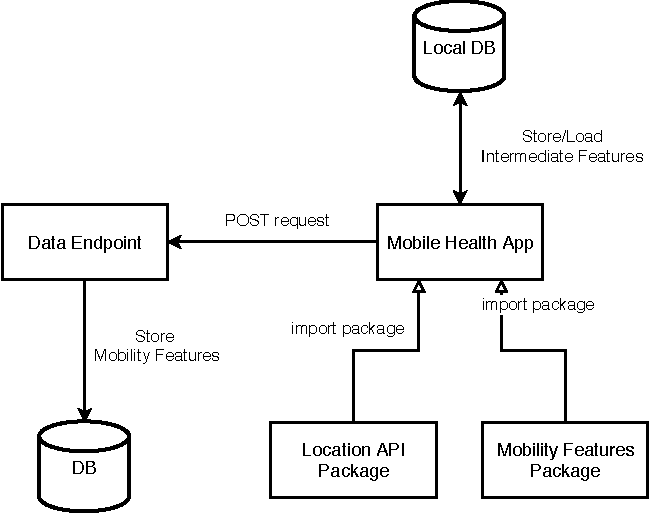
\includegraphics[width=0.5\textwidth]{images/diagrams/data-flow.pdf}
    \caption{Component diagram for a use case of the Mobility Feature Package}
    \label{fig:component-diagram}
\end{figure}

The general idea is to provide an API that allows the application programmer to regularly compute mobility features, for example by means of a trigger. The reason for not including the location tracking within the Mobility Features Package itself, is to make it more modular and easier to maintain. If it was to include a Location package, it could possibly end up conflicting with other location packages the application developer is already using for other parts of their application, and the API would be a lot more convoluted by having to deal with permission requests. The upside to including the location package would however be that the usage of the package becomes easier and a lot of complexity is concealed from the application programmer. 

Concretely, an application programmer will have to start location tracking using their package of choice which will have its own \textit{Data Transfer Object} (DTO) which stores location data, i.e. latitude, longitude and a timestamp. The content of this DTO is then simply transferred to the DTO of the \textit{Mobility Features Package}, namely \textit{SingleLocationPoint} which takes a small amount of code but provides great flexibility in terms of packages used and prevents unnecessary dependency issues. While the Location API was chosen to be external from the package, it was however chosen to include the saving and loading of Stops and Moves in the first iteration. The reason for this is that, in contrast to transferring data from one DTO to another, it takes a lot of manual code to write the store- and load procedure for saving objects on the device and for serializing objects and saving them to a file, no external packages are needed - just the local file system. This means no dependency issues are likely to arise as a result of including the serialization (include save and load) in the package.
